\section{Introduction}\label{intro}


Air quality, while not always noticeable, is a very important environmental measurement which should not be ignored. Air pollution levels are rising in many places across the planet, with cities such as Beijing, China, having levels as high as 886 $\upmu$gm$^{-3}$ of PM2.5 (small particles less than 2.5 microns in diameter)~\cite{beijinghightwitter}. In order to combat these life endangering numbers, we must first have accurate measurements of the pollutants. In Edinburgh, Scotland,  the levels of PM2.5 appear to hover around 8-10 $\upmu$gm$^{-3}$, occasionally spiking up towards 40-50 $\upmu$gm$^{-3}$~\cite{pm2point5inscotland}, and so is generally much less of a problem. This decrease in Edinburgh is similar with most other air pollutants, however Edinburgh can still be used to test and evaluate pollutant measuring and collection models. 

\begin{figure}[H]
    \begin{center}
        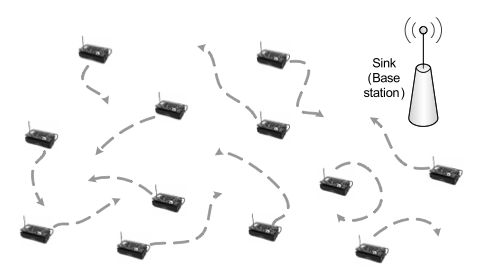
\includegraphics[scale=0.6]{./images/mpp1/BusModel.png}
        \caption{Example of sensors moving around with a static access point}
        \label{fig:busmodel}
    \end{center}
\end{figure}

This project has the aim of evaluating the suitability of using sensors mounted on mobile entities, in this case buses, combined with an optimised data retrieval technique, to measure air quality across the city of Edinburgh in an efficient and responsive manner. Figure~\ref{fig:busmodel} illustrates the model which will be used. With this there are a number of challenges and problems which must be solved including, but not limited to, creating definitions of ``air quality'', how to build a sensor, how to collect the data and how to represent collected data. 

The remainder of this report is laid out as follows. In section~\ref{preliminary} I highlight some of the more difficult problems which needed to be solved. Section~\ref{calibration} discusses how to best calibrate the sensors for the task at hand. Data collection is covered in section~\ref{datacollection} and the representation of said data is covered in section~\ref{geostatistics}. Finally my work plan for the coming year is covered in section~\ref{workplan}.

